
\section{Problemformulering}
At designe og fremstille et éndimensionelt vognmonteret omvendt pendul, der ved hjælp af regulering skal kunne fastholde en forudbestemt vinkel af pendulet, samt at kunne kompensere for udefrakommende påvirkninger. 

\subsection{Formål}
Formålet med projektet er, at forene de opnåede fagligheder fra undervisningen på 3. semester. 
Alle fag fra undervisningen indgår i projektet, og er henholdsvis elektronik, elektromagnetisme, regulering, kredsløbsteknik og matematik.
Det er dermed ønskeligt, at eftervise teorien med praksis. 


\subsection{Krav til rapporten stillet i projektoplæg}
Måling og generering af elektromagnetiske felter kombineret med analog signalbehandling.
\begin{itemize}
\item Der skal udføres et projekt i overensstemmelse med semestertemaet.
\item Projektet skal indeholde fagligheder fra alle teorifagene. Fra elektrofysikken skal
magnetiske felter behandles.
\item Der skal foretages en grundig problemanalyse, der munder ud i en klar og entydig
problemformulering.
\item Produktet skal i videst mulig omfang baseres på lagerførte varer.
\end{itemize}

\subsection{Selvvalgte krav til produktet} \label{afs:kravspecifikation}
Udover de stillede projektkrav, er der også givet nogle selvvalgte krav til produktet. Disse krav er estimeret løbende i projektets fremskriden.
\begin{itemize}
\item Pendulet skal altid starte i ligeposition, og må kun påvirkes små udefrakommende krafter.
\item (Masser af systemet)
\item Systemet skal kunne drives af et/to batteri(er)
\item Sensoren skal være induktiv
\end{itemize}

\subsection{Problemstilling}
Følgende problemstillinger ønskes besvaret:
\begin{itemize}
\item Første
\item Anden
\end{itemize}

\subsection{Projektafgrænsning}
Følgende medtages ikke i rapporten og afgrænser projektarbejdet:
\begin{itemize}
\item Systemet skal kun virke i én retning (dimension)
\item Der ses bort fra fysisk beskrivelse af elektromotoren.
\item Der ses bort fra beskrivelsen af motorstyringen.
\item Vogn samt tilhørende motor, hjul og gearing overtages fra tidligere projekt.
\end{itemize}

\section{Løsningsmodel}
Blokdiagrammet her ?
\husk{JJ}{Del diagram af system og signalvej ?}

\section{Læsevejledning}
Rapportens læsevejledning...\\
Naturlig indførelse i emnet

\section{Arbejdsmetode}
Noter til arbejdsmetoden.
\begin{itemize}
	\item Iterativ planlægning
	\item ugentlige status møder hvor der opsummeres
	\item fleksibel opgave styring, for maksimal udnyttelse af ressourcer 
	\item To-Do lister
\end{itemize}

\section{Blokdiagram}
\begin{figure}[h!]
	\centering
	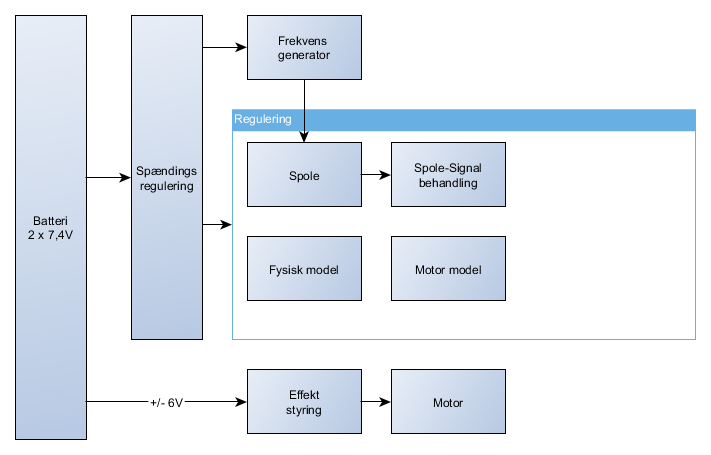
\includegraphics[width=.9\textwidth]{diagram/blokdiagram1.png}
	\caption{System blokdiagram.}
	\label{fig:blockdiagram1}
\end{figure}
\FloatBlock




